\chapter {Interfacing a Light Dependent Resistor}
\thispagestyle{empty}
\label{ldr}

\newcommand{\LocLDRfig}{\Origin/user-code/ldr/figures}
\newcommand{\LocLDRscicode}{\Origin/user-code/ldr/scilab}
\newcommand{\LocLDRscibrief}[1]{{\tt
      \seqsplit{Origin/user-code/ldr/scilab/#1}},
  see \fnrefp{fn:file-loc}}
\newcommand{\LocLDRardcode}{\Origin/user-code/ldr/arduino}
\newcommand{\LocLDRardbrief}[1]{{\tt
      \seqsplit{Origin/user-code/ldr/arduino/#1}},
  see \fnrefp{fn:file-loc}}

%%%%%%%%%python
\newcommand{\LocLDRpycode}{\Origin/user-code/ldr/python}
\newcommand{\LocLDRpybrief}[1]{{\tt \seqsplit{%
        Origin/user-code/ldr/python/#1}}, see \fnrefp{fn:file-loc}}
%%%%%%python

%%%%%%%%%julia starts
\newcommand{\LocLDRjuliacode}{\Origin/user-code/ldr/julia}
\newcommand{\LocLDRjuliabrief}[1]{{\tt \seqsplit{%
        Origin/user-code/ldr/julia/#1}}, see \fnrefp{fn:file-loc}}
%%%%%%julia ends

%%%%%%OpenModelica Starts
\newcommand{\LocLDROpenModelicacode}{\Origin/user-code/ldr/OpenModelica}  %added for OpenModelica
\newcommand{\LocLDROpenModelicabrief}[1]{{\tt \seqsplit{%
        Origin/user-code/led/OpenModelica/#1}}, see \fnrefp{fn:file-loc}} % added for OpenModelica

%%%%%OpenModelcia Ends


A Light Dependent Resistor (LDR) or Photoresistor is a light sensitive
semiconductor device whose resistance varies with the variation in the
intensity of light falling on it. As the intensity of the incident
light increases, resistance offered by the LDR decreases. Typically,
in dark, the resistance offered by an LDR is in the range of a few
mega ohms. With the increase in light intensity, the resistance
reduces to as low as a few ohms.   

An LDR is widely used in camera shutter control, light intensity
meters, burglar alarms, street lighting control, automatic emergency
lights, etc. In this chapter we shall interface an LDR with the
\arduino\ board.  

\section{Preliminaries}
A typical LDR and its symbolic representation are shown in
\figref{fig:ldr} and \figref{fig:ldrsym} respectively. The Shield
provided with the kit has an LDR mounted on it.  The LDR mounted on
the Shield looks exactly like the picture in \figref{fig:ldr},
although, the picture looks a lot larger.  This LDR is connected
to the analog pin 5 of the \arduino\ board. The connections for this
experiment are shown in \figref{fig:ldrconn}. However, the user
doesn't need to connect any wire or component explicitly.

\begin{figure}
  \centering
  \subfloat[Pictorial representation of an LDR]{
    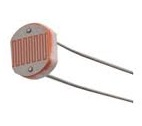
\includegraphics[width=\smfig]{\LocLDRfig/ldr.jpg}
    \label{fig:ldr}} \hfill
  \subfloat[Symbolic representation of an LDR]{
    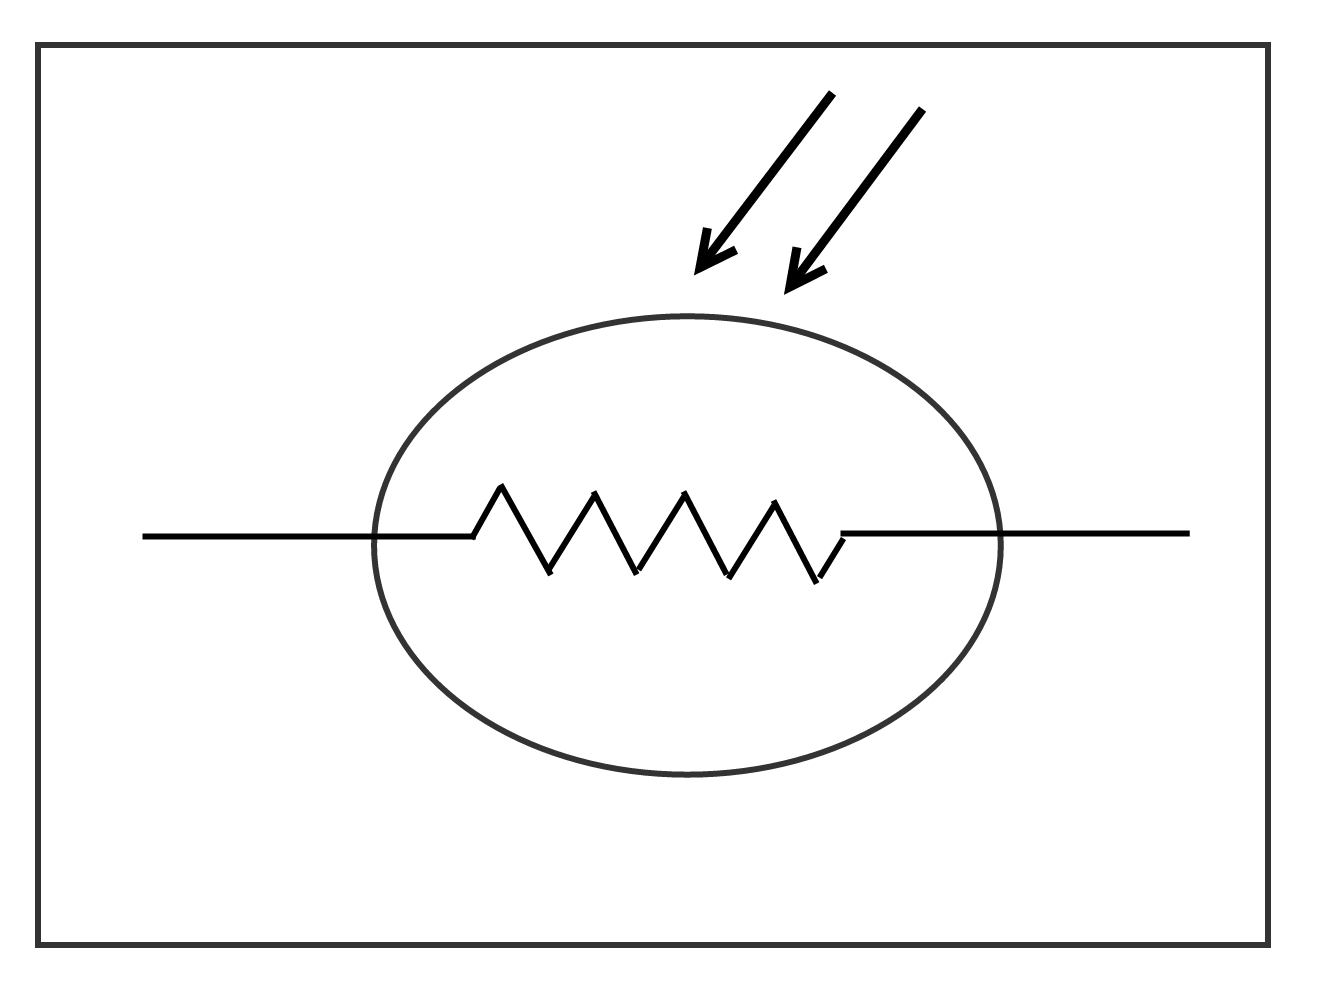
\includegraphics[width=\smfig]{\LocLDRfig/ldr_sym.png}
    \label{fig:ldrsym}}
  \caption{Light Dependent Resistor}
\end{figure}

\begin{figure}
  \centering
  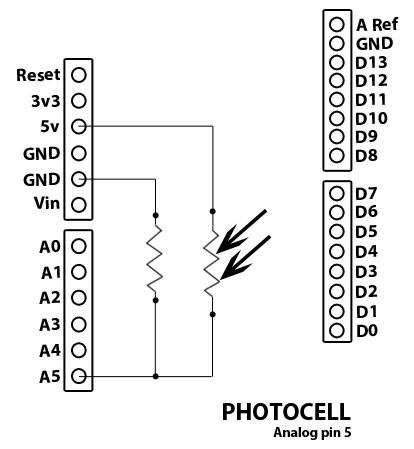
\includegraphics[width=\smfig]{\LocLDRfig/ldr-conn.png}
  \caption{Internal connection diagram for the LDR on the Shield}
  \label{fig:ldrconn}
\end{figure}

The LDR mounted on the Shield is an analog sensor. Hence, the analog voltage, corresponding to the changing resistance, across its terminals needs to be digitized before being sent to the computer. This is taken care of by an on-board Analog to Digital Converter (ADC) of ATmega328 microcontroller on the \arduino\
board. ATmega328 has a 6-channel, 0 through 5, 10 bit ADC. Analog pin
5 of the \arduino\ board, to which the LDR is connected, corresponds
to channel 5 of the ADC.  As there are 10 bits, 0-5V readings from LDR
are mapped to the ADC values from 0 to 1023. 

LDR is a commonly available sensor in the market. It costs about
Rs. 100. There are multiple manufacturers which provide commercial
LDRs.  Some examples are VT90N1 and VT935G from EXCELITAS TECH, and
N5AC501A085 and NSL19M51 from ADVANCED PHOTONIX. 

\section{Connecting an LDR using breadboard}
This section is useful for those who either don't have a Shield or don't want to use the Shield
for performing the experiments given in this chapter.

A breadboard is a device for holding the components of a circuit and connecting 
them together. We can build an electronic circuit on a breadboard without doing any 
soldering. To know more about the breadboard and other electronic components, 
one should watch the Spoken Tutorials on Arduino as published on
  {\tt https://spoken-tutorial.org/}. Ideally, one should go through all the
tutorials labeled as Basic. However, we strongly recommend the readers should
watch the fifth and sixth tutorials, i.e., {\tt First Arduino Program} and 
  {\tt Arduino with Tricolor LED and Push button}.

\begin{figure}
  \centering
  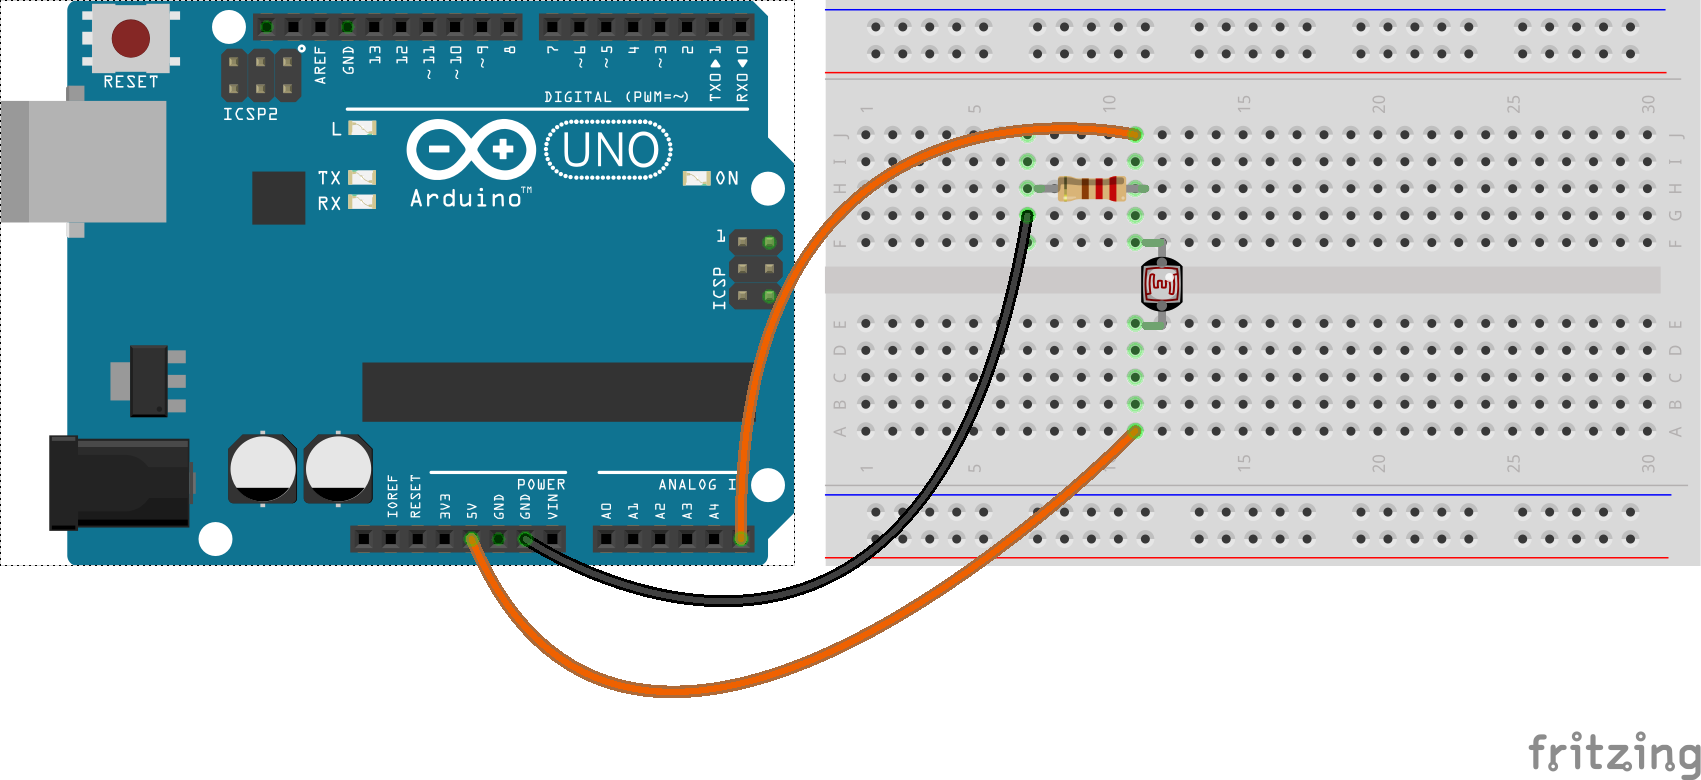
\includegraphics[width=\textwidth]{\LocLDRfig/LDR.png}
  \caption{An LDR to read its values with \arduino\ using a breadboard}
  %\redcolor{connected on pin no. D12}}
  \label{fig:ard-ldr}
\end{figure}

In case you have an LDR, and you want to connect it with \arduino\ on a breadboard, 
please refer to \figref{fig:ard-ldr}. The connections given in this figure can be 
used to read the voltage values from an LDR connected to the analog pin 5 on 
\arduino\ board. As shown in \figref{fig:ard-ldr}, one leg of the LDR is connected 
to 5V on \arduino\ and the other leg to the analog pin 5 on \arduino. A resistor is also connected to the same leg and grounded. 
From \figref{fig:ldrconn} and \figref{fig:ard-ldr}, one can infer that a resistor 
along with the LDR is used to create a voltage divider circuit. The varying 
resistance of the LDR is converted to a varying voltage. Finally, this voltage is used 
by the analog pin 5 of \arduino\ in its logic. 

The connections shown in \figref{fig:ard-ldr-led} can be used to control an RGB LED, 
depending on the voltage values from the LDR. As shown in \figref{fig:ard-ldr-led}, 
digital pin 11 on \arduino\ is connected to the leftmost leg of the RGB LED. Rest of the connections
are same as that in \figref{fig:ard-ldr}. 

\begin{figure}
  \centering
  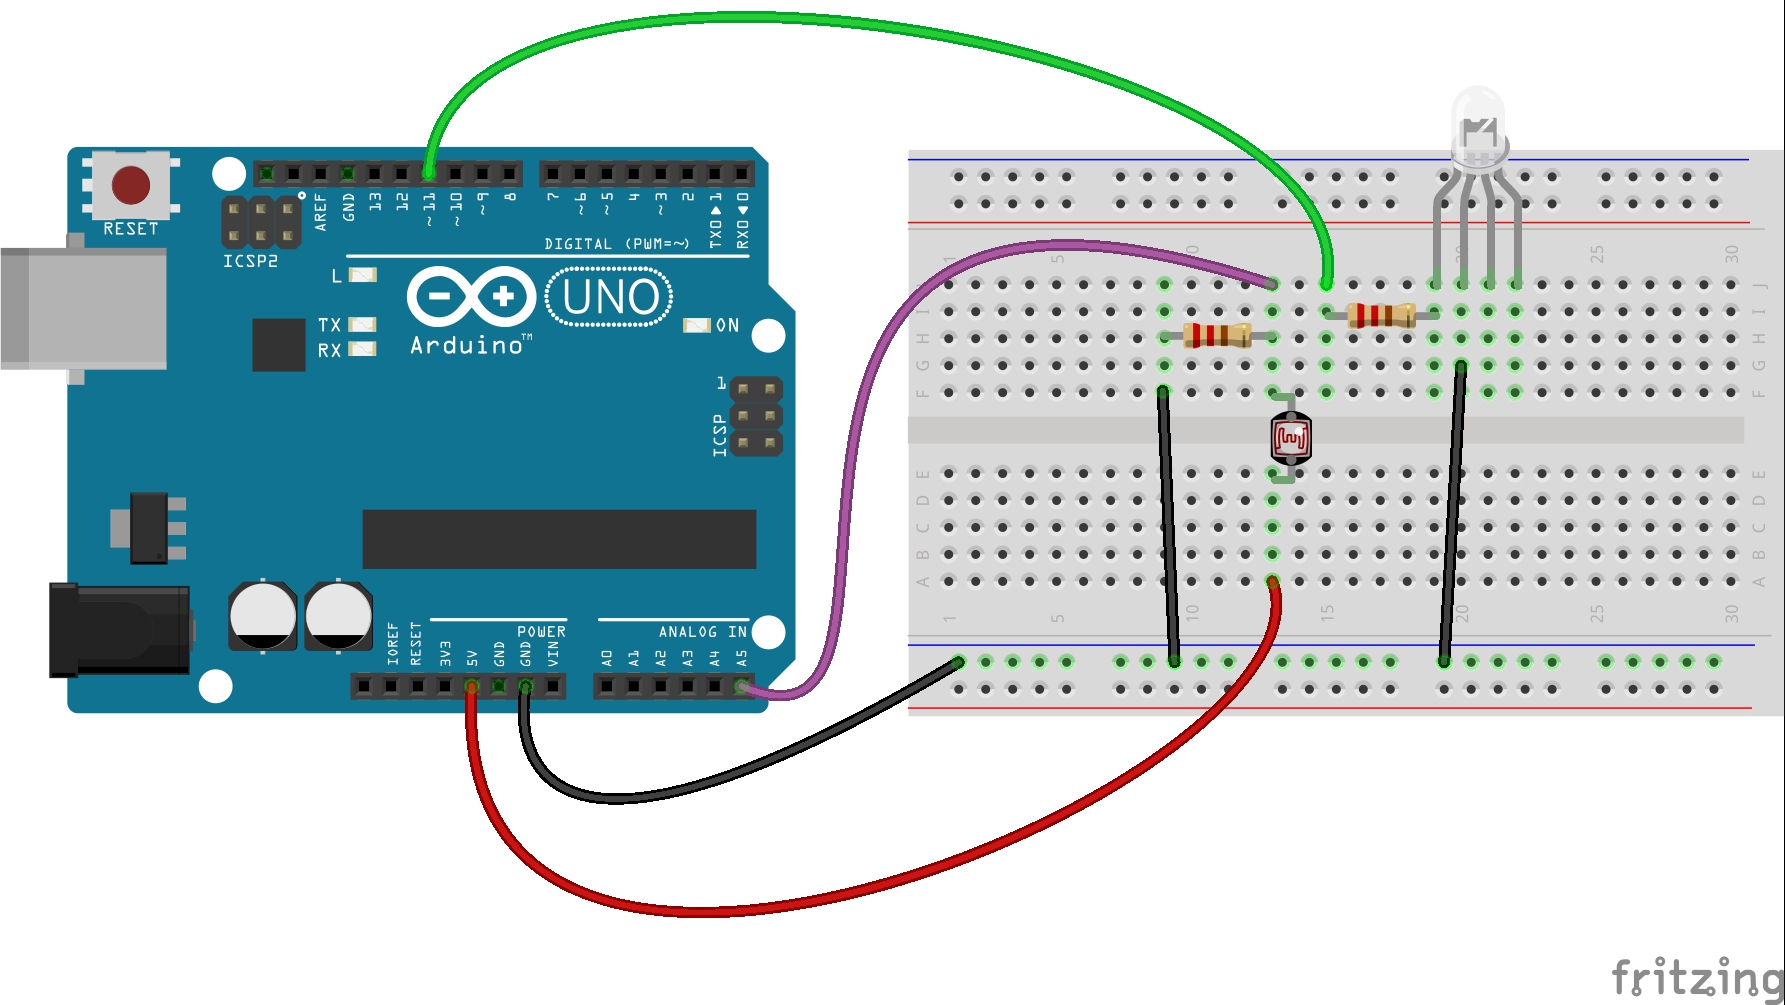
\includegraphics[width=\textwidth]{\LocLDRfig/LDR-led-dark-color-wires.jpg}
  \caption{An LDR to control an LED with Arduino Uno using a breadboard}
  %\redcolor{connected on pin no. D12}}
  \label{fig:ard-ldr-led}
\end{figure}


\section{Interfacing LDR through Arduino IDE}
\subsection{Interfacing the LDR}
In this section, we shall describe an experiment that will help 
to read the voltage values from an LDR connected to the analog pin 5 
of the \arduino\ board. Later, the read values will be used to change the state of an LED.  The Shield has to be attached to the \arduino\ board
before doing these experiments and the \arduino\ needs to be connected to the computer 
with a USB cable, as shown in \figref{arduino}. The reader should go through the
instructions given in \secref{sec:ard-start} before getting started.

\begin{enumerate}
  \item A simple code to read the LDR values is given in
        \ardref{ard:ldr-read}. As discussed earlier, the 0-5V LDR readings
        are mapped to 0-1023 through an ADC. The 
        %\redcolor{Arduino IDE}\ 
        Arduino IDE
        based command for the analog read functionality is given by,
        \lstinputlisting[firstline=6,lastline=6]
        {\LocLDRardcode/ldr-read/ldr-read.ino} where {\tt A5} represents the
        analog pin 5 to be read and the read LDR values are stored in the
        variable {\tt val}.  The read values are then displayed using,
        \lstinputlisting[firstline=7,lastline=7]
        {\LocLDRardcode/ldr-read/ldr-read.ino} The delay in the code  
        \lstinputlisting[firstline=8,lastline=8]
        {\LocLDRardcode/ldr-read/ldr-read.ino} is added so that the readings
        do not scroll away very fast.  The entire reading and display
        operation is carried out 50 times. 
        
        To observe the values, one has to open the {\tt Serial Monitor} of
        the Arduino IDE.  The numbers displayed are in the range 0 to 1023
        and depend on the light falling on the LDR.  If one does the
        experiment in a completely dark room, the reading will be 0.  If on
        the other hand, a bright light, say for instance the torch light
        from mobile, is shined, the value displayed is close to 1023.  One
        will get intermediate values by keeping one's finger on the LDR. 
        While running this experiment, the readers must keep their fingertips on the LDR and
        observe the change in values being printed on the
          {\tt Serial Monitor} of Arduino IDE.
        
  \item This experiment is an extension of the previous
        experiment. Here, depending the resistance of the LDR, we will
        turn the red LED on.  The program for this is available at
        \ardref{ard:ldr-led}.  The value of LDR is read and stored in {\tt
            val}.  In case it is below some threshold (like 300 in \ardref{ard:ldr-led}), 
        it puts a high in pin number 11.  From \secref{sec:led-pril}, 
        one can note that this pin is for the red LED.  If the LDR value is below 300, 
        the red LED will be on, else, it will be turned off.  While running this experiment, the readers 
        must keep their fingertips on the LDR so that the threshold is achieved. Accordingly, 
        they can observe whether the red LED is turned on. 
\end{enumerate}

\begin{exercise}
  Carry out the following exercise:
  \begin{enumerate}
    \item Carry out the experiment in a dark room and check what values
          get displayed on the {\tt Serial Monitor}.
    \item Carry out the experiment with the torch light from the mobile
          phone shining on the LDR.
  \end{enumerate}
\end{exercise}

\subsection{Arduino Code}
\label{sec:ldr-arduino-code}
\addtocontents{ard}{\protect\addvspace{\codclr}}

\begin{ardcode}
  \acaption{Read and display the LDR values}
  {Read and display the LDR values.  Available at
    \LocLDRardbrief{ldr-read/ldr-read.ino}.}
  \label{ard:ldr-read}
  \lstinputlisting{\LocLDRardcode/ldr-read/ldr-read.ino}
\end{ardcode}

\begin{ardcode}
  \acaption{Turning the red LED on and off}
  {Turning the red LED on and off.  Available at
    \LocLDRardbrief{ldr-led/ldr-led.ino}.}
  \label{ard:ldr-led}
  \lstinputlisting{\LocLDRardcode/ldr-led/ldr-led.ino}
\end{ardcode}

